% A link in a node with colorlinks: the link's end is a whatsit, so the
% node's \unskip takes nothing and its size stays known.
\documentclass{article}
\usepackage{tikz}
\usetikzlibrary{arrows.meta}
\usepackage{hyperref}
\hypersetup{colorlinks=true,urlcolor=blue}
\begin{document}
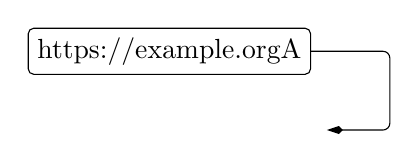
\begin{tikzpicture}
\node[draw,rounded corners=2pt] (a) at (0,0) {\href{https://example.org}{A}};
\draw[rounded corners=2.5pt,-Kite] (a.east) -- ++(1,0) |- (2,-1);
\end{tikzpicture}
\gdef\SatexReachedEnd{}
\end{document}
